\documentclass[addpoints]{exam}

\printanswers
\bracketedpoints

\usepackage{amsmath}
\usepackage{amssymb}
\usepackage{graphicx}
\usepackage{color}



\footer{ELE6209A}{Page \thepage\ de \numpages}{Été 2022}

%\input{commands.tex}

\begin{document}

\begin{coverpages}
\coverfooter{ELE6209A}{Page de couverture}{Été 2022}

%\title{Examen Final\\ ELE3202 - Introduction \`a l'automatisation\\
%\vspace{0.5cm}
%\large D\'epartement de g\'enie \'eletrique\\\'Ecole Polytechnique de Montr\'eal}
%\date{Vendredi 19 avril 2013\\
%\vspace{0.2cm}
%Dur\'ee: 2h30, de 13h30 \`a 16h00}
%\maketitle

\begin{center}
\makebox[\textwidth]{\Large{ELE6209A - Systèmes de navigation}} 
\vspace{0.5cm}

\makebox[\textwidth]{\large{Département d'ingénierie électrique}}

\makebox[\textwidth]{\large{\'Ecole Polytechnique de Montr\'eal}}

\vspace{0.5cm}
\makebox[\textwidth]{\large{Été 2022}}


\end{center}

\begin{center}
\makebox[\textwidth]{Instructor: J\'er\^ome Le Ny} \\ %, \textbf{poste 4886}} \\
\vspace{0.5cm}
\fbox{\fbox{\parbox{5.5in}{\centering
Answer the questions on the exam book. \\%R\'epondre aux questions sur le cahier d'examen distribu\'e. \\
Always clearly and concisely explain the reasoning leading to your answers. Numerical answers without
explanations can be counted as wrong, even if the result is correct. \\ %Expliquer clairement votre raisonnement pour arriver \`a vos r\'eponses. \\
Your answers can be written in English or French. \\%Les r\'eponses peuvent \^etre r\'edig\'ees en fran\c{c}ais ou en anglais.\\
You do not have to answer the problems in the order provided. However, you must group your answers
to the questions of the same problem together. \\
If relevant, the units in which your numerical answers are expressed must be stated.
Manage your time carefully: the points attributed to each question should give you an indication on how much
time to spend on them. Not all questions are of the same difficulty. I recommend you first skim through the exam
to identify the problems you are most comfortable with. \\ 
\vspace{0.5cm}
Documents allowed: instructor's lecture notes and slides. \\%Une calculatrice non programmable est permise.
A non-programmable calculator is allowed. \\
Please return the question sheet at the end.
}}}
\end{center}

\vspace{2cm}
\begin{center}
\textcolor{red}{\textbf{SOLUTION}}
\end{center}

\vspace{3cm}
\begin{center}
\gradetable[h][questions]
\end{center}


\newpage
\begin{center}
- This page intentionally left blank -
\end{center}

\end{coverpages}





%%%%%%%%%%%%%%
% Start of the exam
%%%%%%%%%%%%%%


\begin{questions}

\question
\begin{parts}
\part[2]  Sachant que la position $[n(t_k),e(t_k)]$ et l'angle $\psi(t_k)$ sont connu à l'instant $t_k$. En se basant sur les équations du chapitre 9.1.2, trouver les équations permettant de calculer $n(t_{k+1}),e(t_{k+1})$ et  $\psi(t_{k+1})$.
\part[1] À l'aide du fichier $Q1.ttt$ modifier la fonction updateOdometry(q,$u_r$,$u_l$). Celle-ci s'occupe de mettre à jours le déplacement du robot dans la simulation. Trois variables sont en entrée.

\begin{itemize}
    \item q : position estimée du robot  $[n,e,\psi]$ dans le repère \{t\}
    \item $u_r$ :  Vitesse de rotation de la roue droite
    \item $u_l$ : Vitesse de rotation de la roue gauche
\end{itemize}
Montrer le graphique de l'erreur entre la trajectoire désirée (ligne verte) et la trajectoire obtenue avec l'odométrie (ligne bleue) pour une simulation de 50 secondes.
\end{parts}


\begin{solution}
\begin{parts}
\part
Vitesses linéaires et angulaires.
\begin{align*}
    u &= \frac{1}{2}(u_l + u_r)\\
    w &= \frac{1}{L}(u_l - u_r)
\end{align*}
Déplacements lineaires et angulaires.
\begin{align*}
    n(t_{k+1}) &= n(t_k) + u\Delta t\cos(\psi(t_k))\\
    e(t_{k+1}) &= e(t_k) + u\Delta t\sin(\psi(t_k))\\
    \psi(t_{k+1}) &= \psi(t_k) + w\Delta t
\end{align*}

\part Graphique représentant l'erreur entre la trajectoire désirée et l'odométrie.

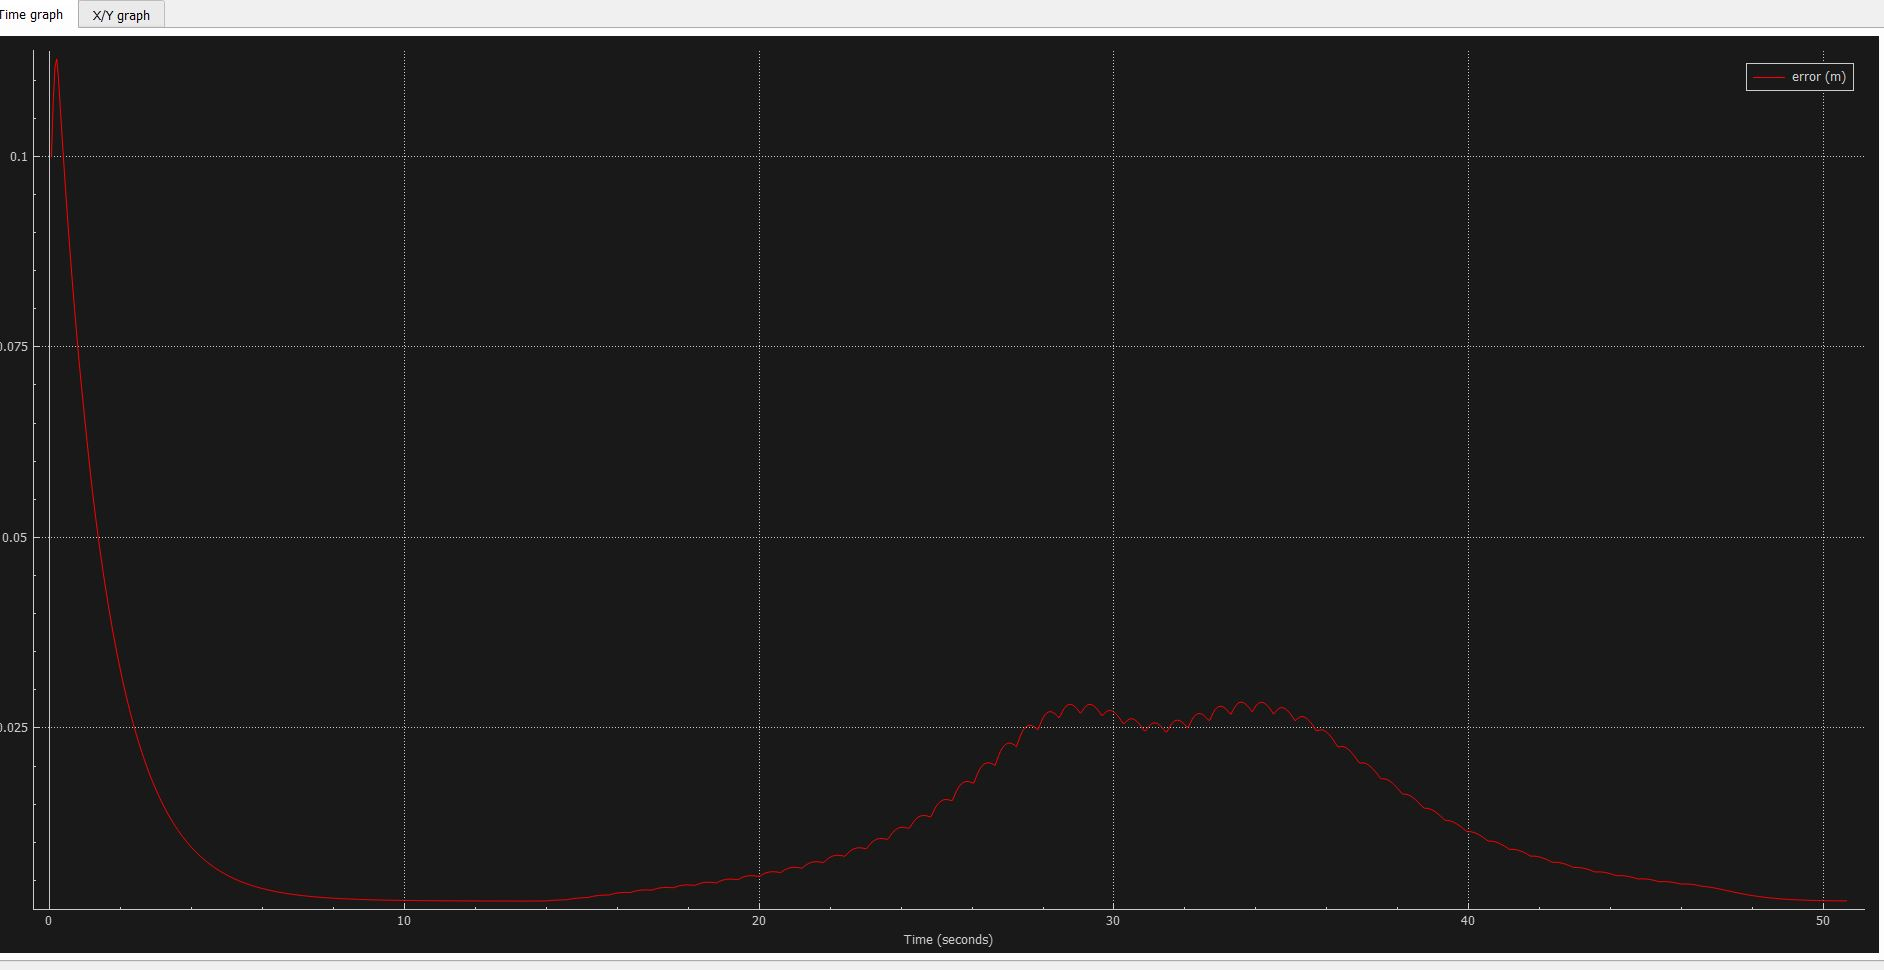
\includegraphics[width=0.5\textwidth]{image/Q1_b.JPG}

\end{parts}
\end{solution}

\question
\begin{parts}
\part[3] À l'aide du fichier $laser\_data.csv$ et en se basant sur la théorie du chapitre 5, trouver la position $[x,y]$ de l'objet se déplacant sur une période de 60 secondes. Le choix du langage de programmation est libre. Utiliser $x_0 = [-1,-1]$ comme premier point de recherche. Le fichier csv est divisé selon les colonnes suivantes:

\begin{table}
    \centering
    \begin{tabular}{|c|c|c|c|}
    \hline 
    X & Y & Distance & Temps\\
    \hline 
    \end{tabular}
    \caption{Colonnes du fichier CSV}
    \label{tab:tab1}
\end{table}

\begin{itemize}
    \item X correspond aux positions x des points repères dans \{t\}
    \item Y correspond aux positions y des points repères dans \{t\}
    \item Distance correspond aux distances entre les points repères et l'objet dans \{t\}
    \item Temps correspond au moment où le point repère est détecté par le laser
\end{itemize}

Montrer le graphique représentant le déplacement $[x,y]$ de l'objet.

\part[1] Implémenter l'algorithm développé en $(a)$. Utiliser le fichier de démarrage $Q2.ttt$. La fonction $findPosition$ doit être modifiée. Celle-ci utilise les données provenant du laser. Elle s'occupe du $position fixing$. Trois variables sont en entrée.

\begin{itemize}
    \item LMpositions : tableau contenant la position de tous les objets détectés par le laser
    \item LMdistance : tableau contenant la distance avec tous les objets détectés par le laser
    \item q : position estimée du robot dans le repère \{t\}
\end{itemize}

La notion de matrice pseudo-inversible devra être utilisée. Montrer les deux graphiques suivant pour une simulation de 60 secondes:
\begin{itemize}
    \item Graphique représentant le déplacement $[x,y]$ du robot 
    \item Graphique d'erreurs entre la position calculée et réelle du robot
\end{itemize}

De plus, donner l'erreur moyenne entre la position calculée et réelle pour la même période.

\end{parts}

\begin{solution}
\begin{parts}

\part
Graphique représentant la position $[x,y]$ de l'objet.

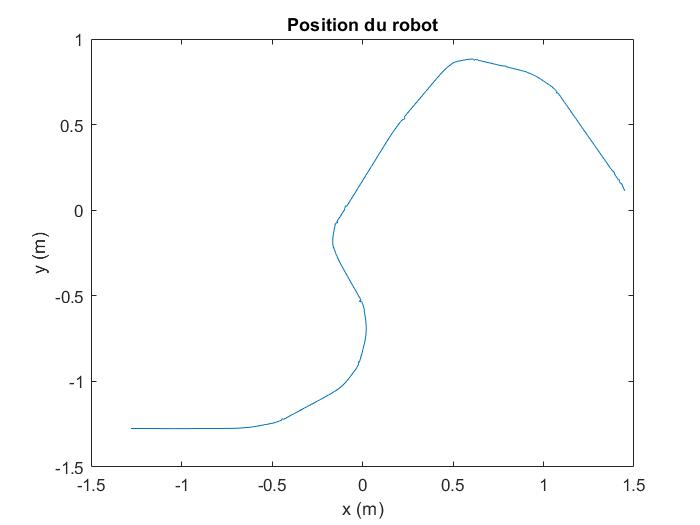
\includegraphics[width=0.5\textwidth]{image/Q2_a.JPG}

\part
Graphique représentant la position $[x,y]$ du robot.

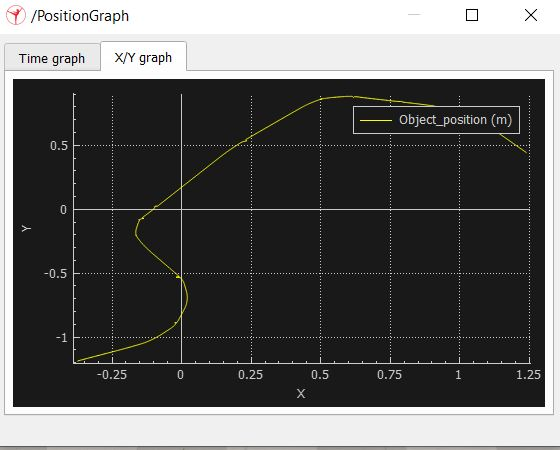
\includegraphics[width=0.5\textwidth]{image/Q2_b1.JPG}

L'erreur moyenne est de $0.00083$ pour 60 une période de secondes.\vspace{3mm}

Graphique représentant l'erreur entre la position calculée et réelle du robot.

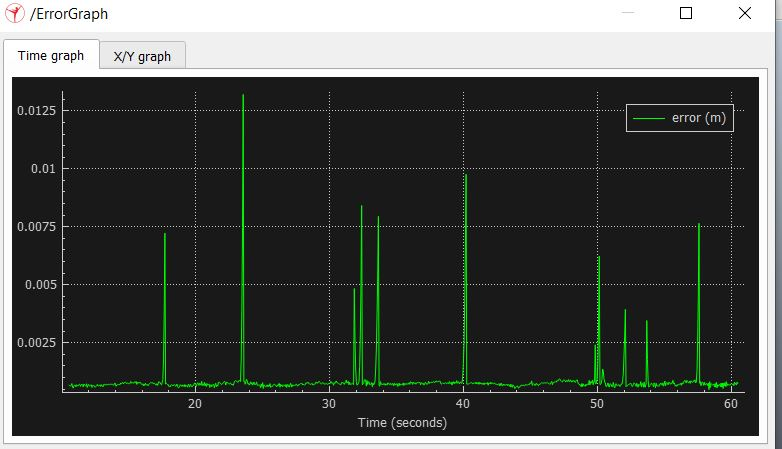
\includegraphics[width=0.5\textwidth]{image/Q2_b2.JPG}

\end{parts}
\end{solution}

\question

Réaliser et comparer 2 filtres de kalman étendu (EKF). Le filtre est utilisé afin de corriger la position estimée avec l'odometrie en utilisant les données lasers.\vspace{3mm}


Les équations d'odométries sont utilisées pour obtenir les équations de navigation:

\begin{align}
    \dot{n} &= \frac{1}{2}\cos{\psi}(R\dot{\theta}_l+w_l + R\dot{\theta}_r+w_r)\\
    \dot{e} &= \frac{1}{2}\sin{\psi}(R\dot{\theta}_l+w_l + R\dot{\theta}_r+w_r)\\
    \dot{\psi} &= \frac{1}{L}(R\dot{\theta}_r+w_r - R\dot{\theta}_l-w_l)
\end{align}

Ici $\dot{\theta}$ correspond à la vitesse de rotation de chaque roue obtenue par odométrie. $w \sim \mathcal{N}(0,\,1\times10^{-2})$, $w_r \perp w_l$.\vspace{3mm}

En linéarisant ($\Delta x = x-\hat{x}$) les équations ci-dessus, on obtient les matrices A et B:

\begin{equation}
    A = \begin{bmatrix}
        0 & 0 & -\frac{R}{2}\sin{\hat{\psi}}(\dot{\theta}_l+\dot{\theta}_r)\\
        0 & 0 & \frac{R}{2}\cos{\hat{\psi}}(\dot{\theta}_l+\dot{\theta}_r)\\
        0 & 0 & 0
        \end{bmatrix}
\end{equation}

\begin{equation}
    B = \begin{bmatrix}
        \frac{1}{2}\cos{\hat{\psi}} & \frac{1}{2}\cos{\hat{\psi}} \\
        \frac{1}{2}\sin{\hat{\psi}} & \frac{1}{2}\sin{\hat{\psi}} \\
        -\frac{1}{L} & \frac{1}{L} 
        \end{bmatrix}
\end{equation}

\begin{align}
    \nonumber R &= 0.0975\\
    \nonumber L &= 0.331
\end{align}


\begin{parts}
\part[1] Selon le modèle linéaire suivant :
\begin{align}
    \Delta\dot{x} &= A(t)\Delta x + B(t)w(t)\\
    \Delta y_k &= C\Delta x_k + D\nu(t)
\end{align}

Trouver les matrices C et D sachant que les mesures ($y_k$) correspondent à la position calculée avec un laser. On suppose ici que le laser donne directement la position du robot dans le repère \{t\}.
\begin{align}
    \nonumber\tilde{n} &= n +\nu_n\\
    \nonumber\tilde{e} &= e +\nu_e
\end{align}

\part[2] Selon le même modèle linéaire que la question (a), trouver les matrices C et D sachant que les mesures ($y_k$) correspondent à l'angle $\theta_i$ et la distance $d_i$ dans le repère \{b\}. Voir schéma suivant :

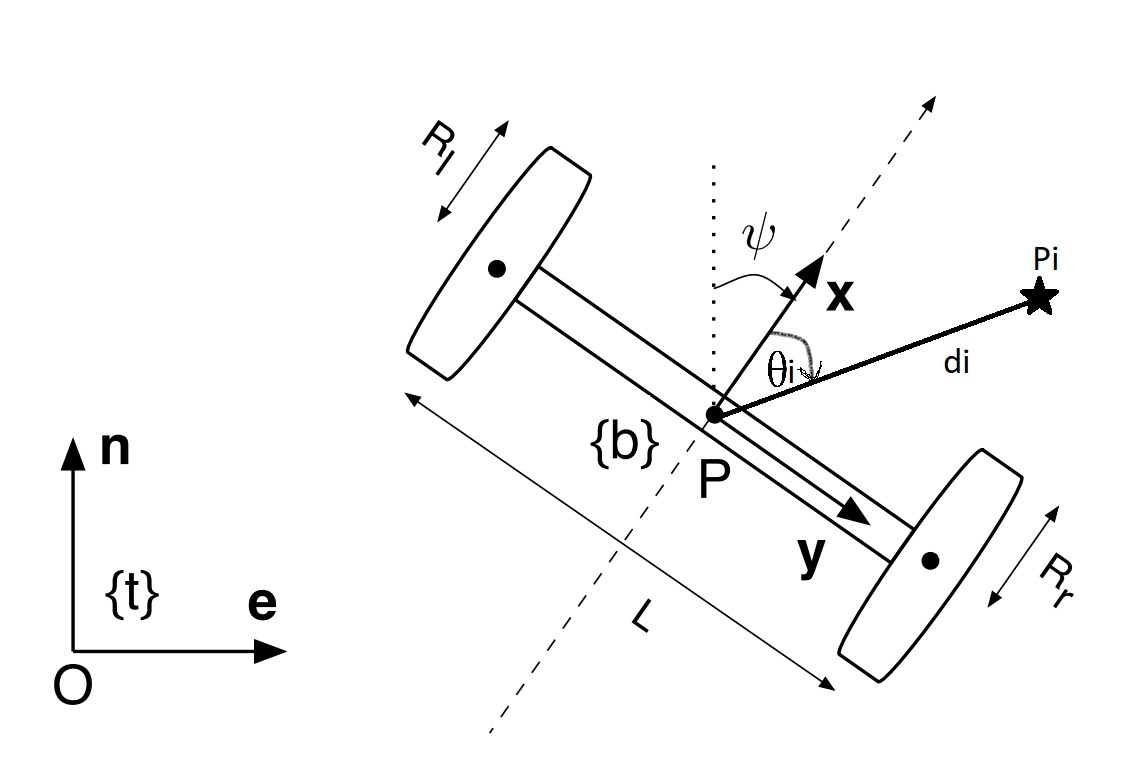
\includegraphics[width=0.7\textwidth]{image/Q3_schema_laser2.jpg}

Ici,
\begin{align}
    \nonumber\tilde{\theta_i} &= \theta_i\\
    \nonumber\tilde{d_i} &= d_i +\nu_i
\end{align}

\part[4] Réaliser, dans le langage de votre choix, deux EKF utilisant les matrices trouvées en (a) et (b). Utiliser les deux fichiers de départ. Le fichier $Laser1$ contient les documents suivants:
\begin{itemize}
    \item   estimated$\_$odometry$\_$position.csv
    \item   laser$\_$data.csv
    \item   odometry$\_$data.csv
    \item   true$\_$pose.csv
\end{itemize}
$laser\_data.csv$ contient la position $x$ et $y$ du robot exprimé dans le repère \{t\} à des instants précis. Le laser utilisé est celui de la question (a).  Le bruit sur les mesures laser est $\nu \sim \mathcal{N}(0,\,5\times10^{-2})$. 
 $\nu_n \perp \nu_e$.\vspace{3mm}

$odometry\_data.csv$ contient les valeurs $u_l$ et $u_r$. Ici $u_i = R\dot{\theta}_i + w_i,\quad i = l,r$\vspace{3mm}
 
$estimated\_odometry\_position.csv$ contient les mesures $x,y$ et $\psi$ calculé à l'aide des équations trouvées au problème 1.\vspace{3mm}

$true\_pose.csv$ contient la position (x,y) ainsi que l'angle $\psi$ réelle du robot.\vspace{3mm}

Le fichier $Laser2$ contient les documents suivants:
\begin{itemize}
    \item   estimated$\_$odometry$\_$position.csv
    \item   laser$\_$data.csv
    \item   lookupTable.csv
    \item   odometry$\_$data.csv
    \item   true$\_$pose.csv
\end{itemize}

Les documents, $estimated\_odometry\_position.csv$, $odometry\_data.csv$ et $true\_pose.csv$ sont identiques à ceux du fichier $Laser1$.\vspace{3mm}

$laser\_data.csv$ contient la distance $d_i$ et l'angle $\theta_i$ dans le repère \{t\} à des instants précis. Le laser utilisé est celui de la question (b).  Le bruit sur les mesures laser $d_i$ est $\nu \sim \mathcal{N}(0,\,5\times10^{-2})$. Le document contient également l'identifiant du point $P_i$ détecté.\vspace{3mm}

$lookupTable.csv$ permet de trouver la position $x$ et $y$ du point $P^t_i$ à l'aide d'un identifiant.\vspace{3mm}

Initialement, le robot se trouve à $\begin{bmatrix} n \\ e \\ \psi\end{bmatrix} = \begin{bmatrix} -1.628 \\ 0 \\ 0\end{bmatrix}$.

Fournir les erreurs moyennes entre l'état $[n,e]$ calculée et réelle à l'aide des EKF. Comparer les résultats des deux EKF et discuter.\vspace{3mm}

\part[2] Réaliser le filtre de votre choix sur Coppeliasim. Utiliser le fichier de départ adéquat ($Q3\_laser1.ttt$ ou $Q3\_laser2.ttt$). Modifier la fonction kalmanFilter. Trois variables sont en entrée.

\begin{itemize}
    \item q : position estimée du robot dans le repère \{t\}
    \item odometryMeasurements : données provenant des encodeurs des roues droites et gauches
    \item positionFixMeasurements : position du robot provenant du laser
\end{itemize}

Montrer l'erreur moyenne ainsi que le graphique de l'erreur entre la position calculée (corrigée à l'aide de l'EKF) du robot vs la position réelle du robot pour une simulation de 90 secondes.

\end{parts}

\begin{solution}
\begin{parts}

\part Le laser mesure la position $[n,e]$ du robot

\begin{align}
    \tilde{n} &= n +\nu_n\\
    \tilde{e} &= e +\nu_e
\end{align}

Ici $\Delta x = x-\hat{x}$:
\begin{equation}
    \nonumber\Delta y_k = \begin{bmatrix} \tilde{n}_k-n_k \\ \tilde{e}_k-e_k \end{bmatrix}\\= \begin{bmatrix} 1 & 0 & 0\\ 0 & 1 & 0 \end{bmatrix}\begin{bmatrix} \Delta n_k \\ \Delta e_k\\ \Delta \psi_k \end{bmatrix} + \begin{bmatrix}1 & 0\\ 0 & 1\end{bmatrix} \begin{bmatrix} \nu_{nk} \\ \nu_{ek} \end{bmatrix}\\
\end{equation}

\begin{align}
    C &= \begin{bmatrix} 1 & 0 & 0\\ 0 & 1 & 0 \end{bmatrix}\\
    D &= \begin{bmatrix}1 & 0\\ 0 & 1\end{bmatrix}
\end{align}

\part Le laser mesure la distance $\theta_i$ et la distance $d_i$ du point $P_i$ dans le repère \{b\}. Solution pour $y_k$ = $P^t_i$:

\begin{align}
    \nonumber\tilde{\theta_i} &= \theta_i\\
    \nonumber\tilde{d_i} &= d_i +\nu_i
\end{align}

\begin{align}
    \tilde{P^b_i} &= \begin{bmatrix}\tilde{d_i}cos(\tilde{\theta_i})\\ \tilde{d_i}sin(\tilde{\theta_i})\end{bmatrix}\\
    y_k &= \hat{P^t_i} = \hat{P^t_b} + \hat{R^t_b}\tilde{P^b_i} = \begin{bmatrix}\hat{n_b} + cos(\hat\psi)\tilde{d_i}cos(\tilde{\theta_i})-sin(\hat\psi)\tilde{d_i}sin(\tilde{\theta_i})\\ \hat{e_b} + sin(\hat\psi)\tilde{d_i}cos(\tilde{\theta_i})+cos(\hat\psi)\tilde{d_i}sin(\tilde{\theta_i})\end{bmatrix}
\end{align}

\begin{equation}
     \nonumber\Delta y_k = \begin{bmatrix} 1 & 0 & -sin(\hat\psi)\tilde{d_i}cos(\tilde{\theta_i})-cos(\hat\psi)\tilde{d_i}sin(\tilde{\theta_i})\\ 0 & 1 & cos(\hat\psi)\tilde{d_i}cos(\tilde{\theta_i})-sin(\hat\psi)\tilde{d_i}sin(\tilde{\theta_i}) \end{bmatrix}\begin{bmatrix} \Delta n_k \\ \Delta e_k\\ \Delta \psi_k \end{bmatrix} + \begin{bmatrix}cos(\hat\psi)cos(\tilde{\theta_i})-sin(\hat\psi)sin(\tilde{\theta_i})\\ sin(\hat\psi)cos(\tilde{\theta_i})+cos(\hat\psi)sin(\tilde{\theta_i})\end{bmatrix} \nu\\   
\end{equation}

\begin{align}
    C &= \begin{bmatrix} 1 & 0 & -sin(\hat\psi)\tilde{d_i}cos(\tilde{\theta_i})-cos(\hat\psi)\tilde{d_i}sin(\tilde{\theta_i})\\ 0 & 1 & cos(\hat\psi)\tilde{d_i}cos(\tilde{\theta_i})-sin(\hat\psi)\tilde{d_i}sin(\tilde{\theta_i}) \end{bmatrix}\\
    D &= \begin{bmatrix}cos(\hat\psi)cos(\tilde{\theta_i})-sin(\hat\psi)sin(\tilde{\theta_i})\\ sin(\hat\psi)cos(\tilde{\theta_i})+cos(\hat\psi)sin(\tilde{\theta_i})\end{bmatrix}
\end{align}


\part Pour l'EKF ($Laser1$), les erreurs moyennes sont :
\begin{align}
    \nonumber n &= -0.0106\\
    \nonumber e &= 0.0602
\end{align}.

Graphique représentant l'erreur entre la position calculée et réelle du robot:

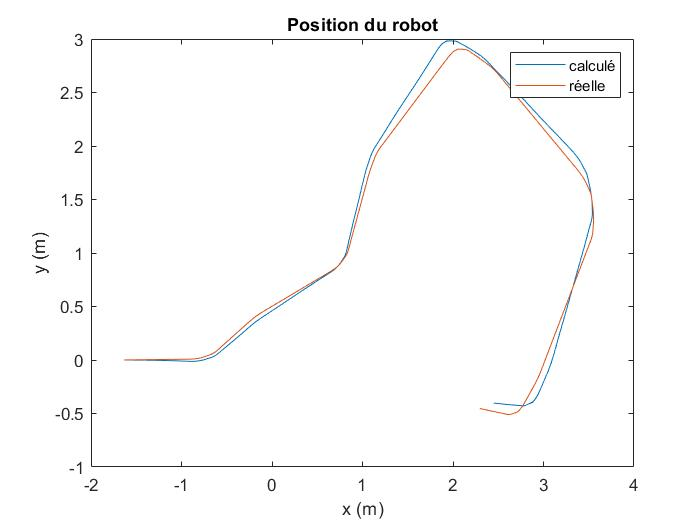
\includegraphics[width=0.5\textwidth]{image/Q3_c1.jpg}

Pour l'EKF ($Laser2$), les erreurs moyennes sont :
\begin{align}
    \nonumber n &= -0.0050\\
    \nonumber e &= 0.0539
\end{align}.

Graphique représentant l'erreur entre la position calculée et réelle du robot:

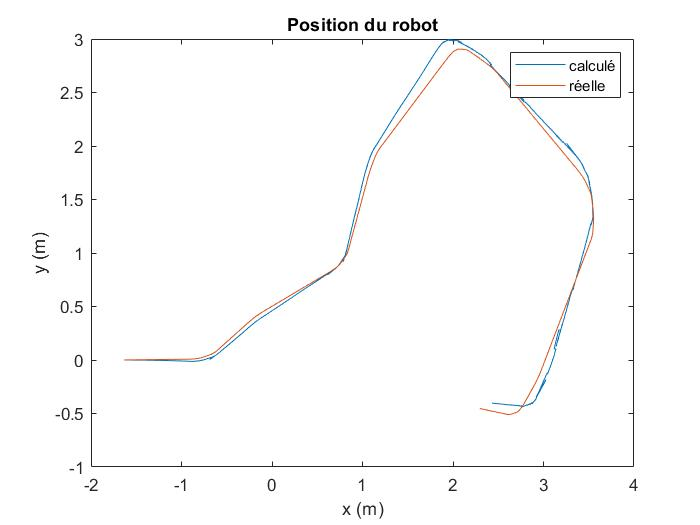
\includegraphics[width=0.5\textwidth]{image/Q3_c2.jpg}

On remarque que les mesures de l'EKF ($Laser1$) ne modifient pas l'angle $\psi$. Pour cette raison les erreurs de $n$ et $e$ de l'EKF ($Laser2$) sont inférieures. Globalement, l'EKF ($Laser2$) semble meilleurs que l'EKF ($Laser1$).

\part Pour l'EKF ($Laser1$), les erreurs moyennes pour une période de 120 secondes sont :
\begin{align}
    \nonumber n &= 0.00110\\
    \nonumber e &= 0.00647
\end{align}

Graphique représentant l'évolution de l'erreur dans le temps (90 secondes):

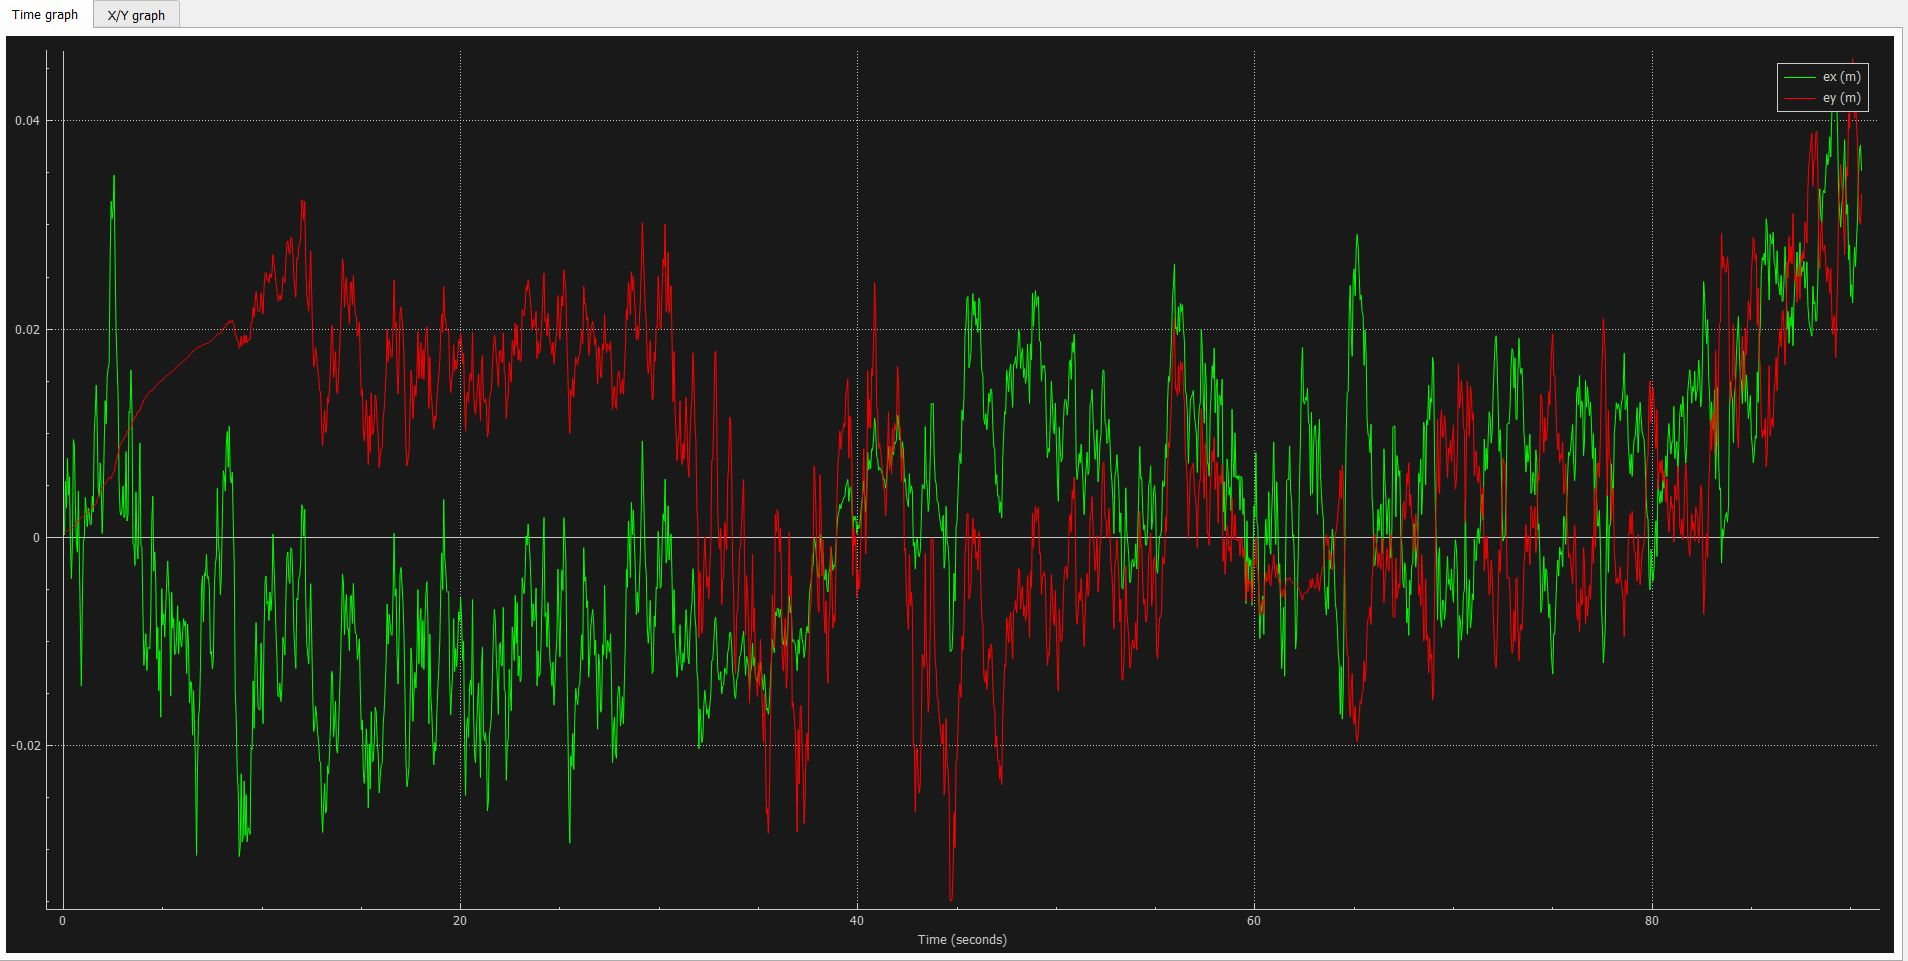
\includegraphics[width=0.5\textwidth]{image/Q3_d1.JPG}

Pour l'EKF ($Laser2$), les erreurs moyennes pour une période de 120 secondes sont :
\begin{align}
    \nonumber n &= 0.01267\\
    \nonumber e &= -0.01081
\end{align}

Graphique représentant l'évolution de l'erreur dans le temps (90 secondes):

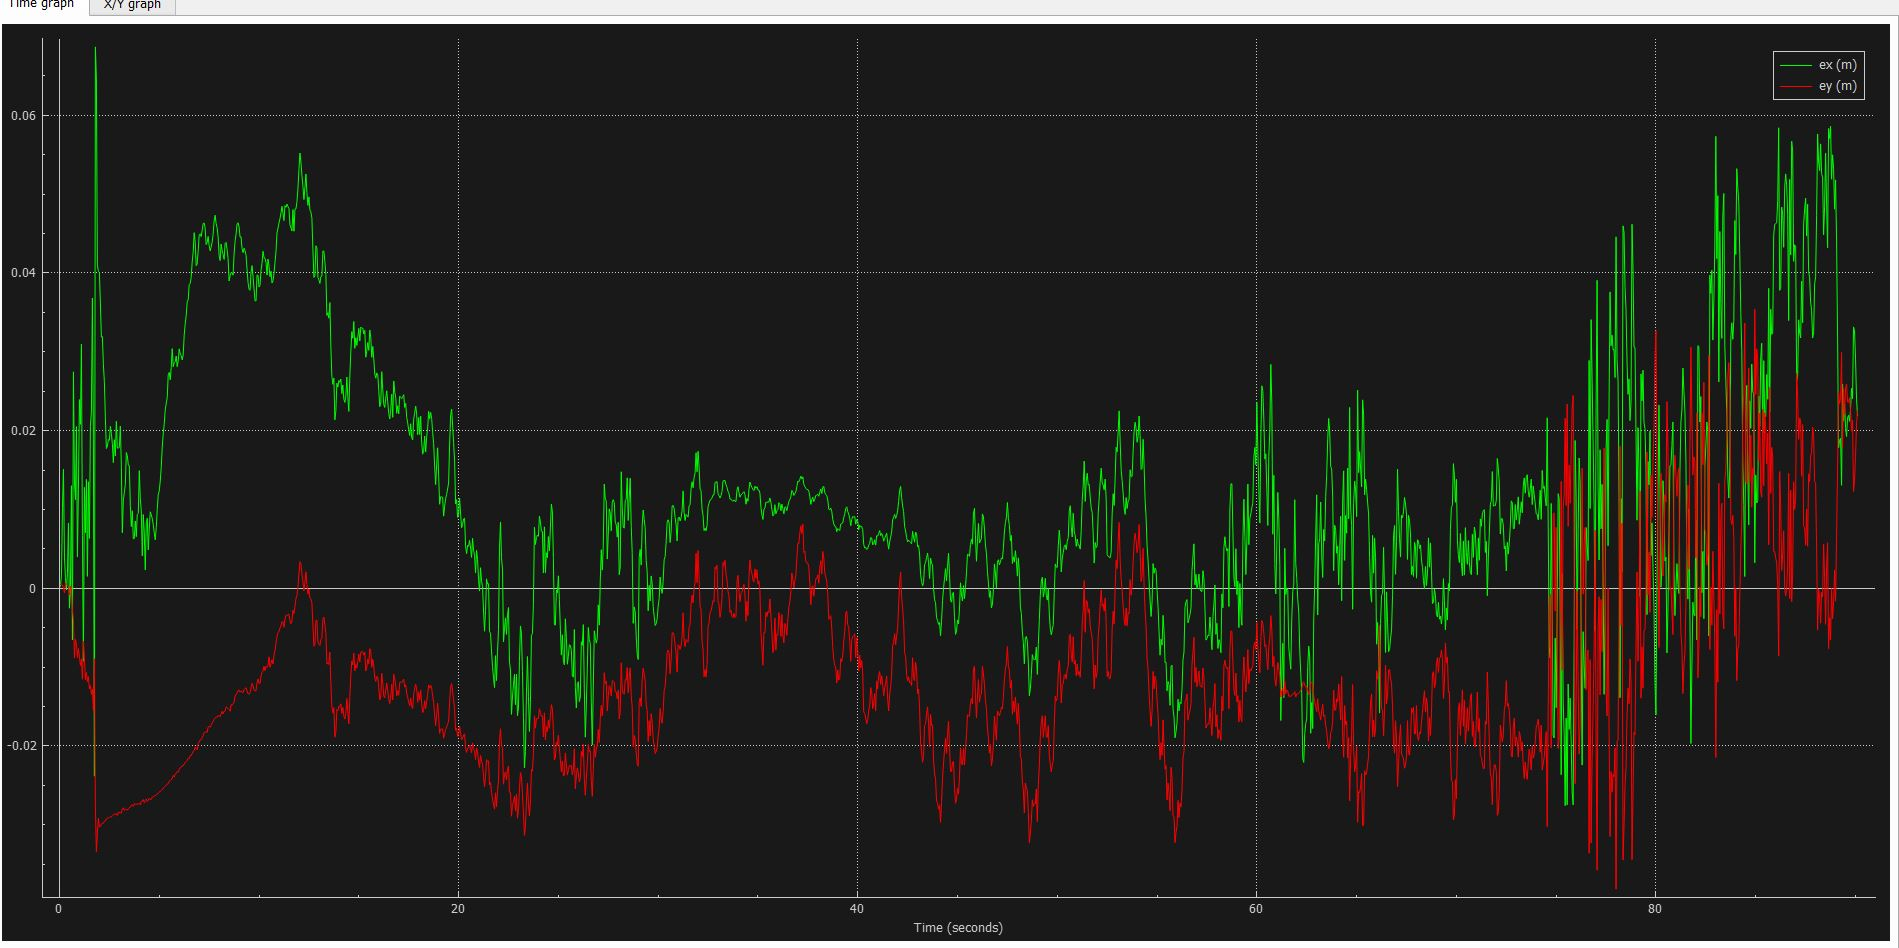
\includegraphics[width=0.5\textwidth]{image/Q3_d2.JPG}

\end{parts}
\end{solution}

\question[4]
Voici le schéma du système:

\begin{figure}[h]
    \centering
    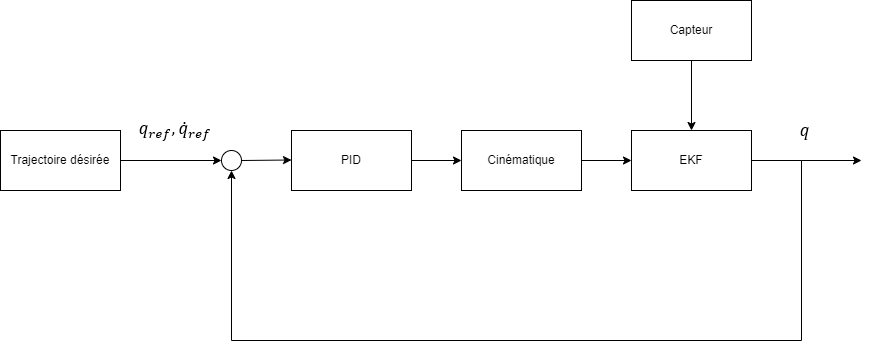
\includegraphics[width=0.80\textwidth]{image/ete_2022_projet_1.drawio.png}
    \caption{Schéma de controle}
    \label{fig:controle}
\end{figure}

Dans le fichier de départ $Q4.ttt$ deux fonctions sont à modifier.
\begin{itemize}
    \item     q = updateOdometry(q,$u_r$,$u_l$)
    \item kResult = kalmanFilter(q,odometryMeasurements,positionFixMeasurements)
\end{itemize}

La fonction $updateOdometry$ s'occupe de mettre à jour le déplacement du robot dans la simulation. Cette fonction représente le module Cinématique du schéma \ref{fig:controle}. Trois variables sont en entrée.

\begin{itemize}
    \item q : position estimée du robot dans le repère \{t\}
    \item $u_r$ :  Vitesse de rotation de la roue droite
    \item $u_l$ : Vitesse de rotation de la roue gauche 
\end{itemize}

La fonction $kalmanFilter$ se charge de la fusion des données par l'intermédiaire de l'EKF. Cette fonction représente le module EKF du schéma \ref{fig:controle}.Trois variables sont en entrée.

\begin{itemize}
    \item q : position estimée du robot dans le repère \{t\}
    \item odometryMeasurements : données provenant des encodeurs des roues droites et gauches
    \item positionFixMeasurements : position du robot provenant du position fixing
\end{itemize}

Le laser est le même que celui utilisé en

Montrer l'erreur moyenne entre la position calculée (corrigée à l'aide de l'EKF) du robot versus la position réelle du robot pour une simulation de 240 secondes. Démontrer aussi, une capture d'écran du trajet effectué suite à une simulation de 240 secondes.

\begin{solution}
L'erreur moyenne est de 0.04214.\vspace{3mm}

Capture d'écran représentant le parcours effectué: 

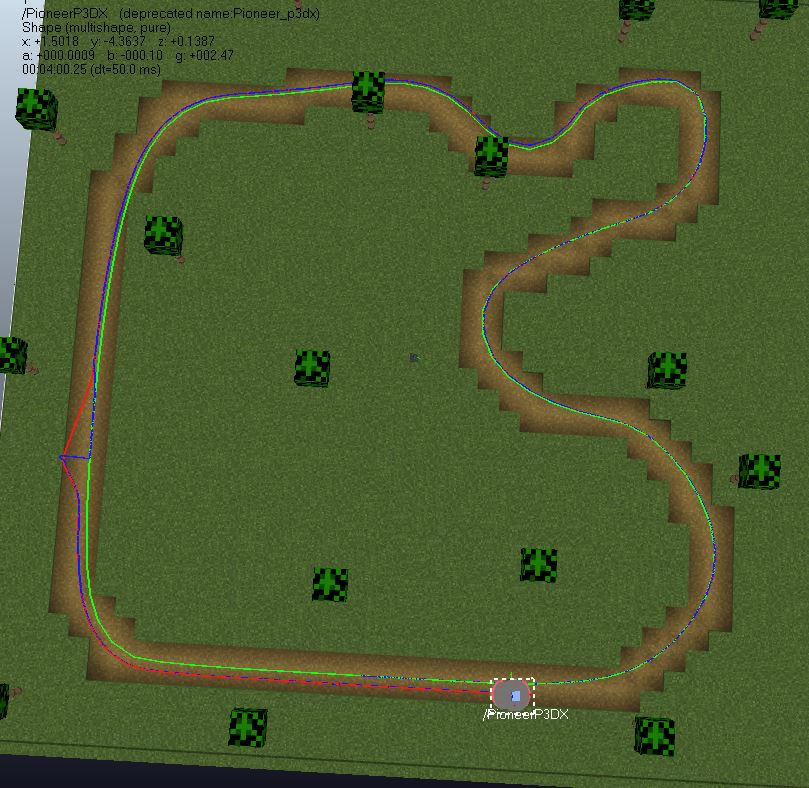
\includegraphics[width=0.8\textwidth]{image/Q4_screenshot.JPG}

\end{solution}

\end{questions}





\end{document}

